% This file defines the command for plotting the Softplus and ReLU functions.
% It can be compiled standalone or included in a larger document.

\ifdefined\ispartofbook
\else
  % --- Standalone Compilation Preamble ---
  \documentclass[tikz, border=10pt]{standalone}
  \usepackage{tikz}
  \usetikzlibrary{arrows.meta}
  \begin{document}
\fi

% --- THE DIAGRAM COMMAND ---
\newcommand{\softplusplot}{%
    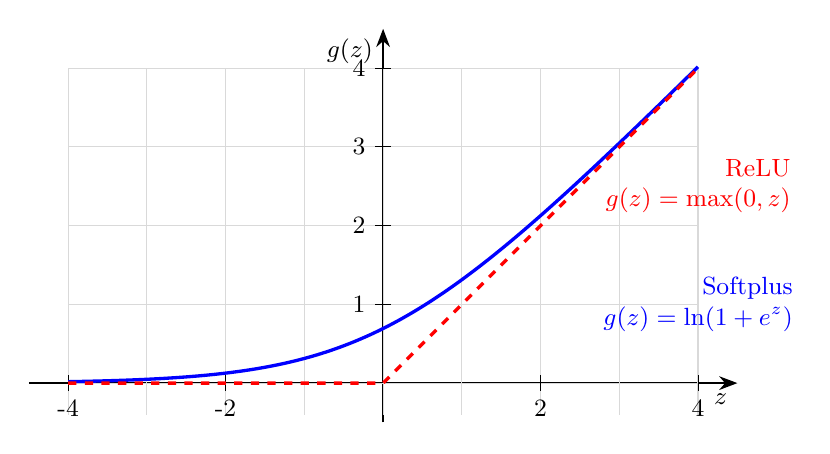
\begin{tikzpicture}[
        font=\sffamily,
        every node/.style={font=\small}
    ]
    % Axes
    \draw[-Stealth, thick] (-4.5,0) -- (4.5,0) node[below left] {$z$};
    \draw[-Stealth, thick] (0,-0.5) -- (0,4.5) node[below left] {$g(z)$};

    % Grid
    \draw[gray!30, thin, step=1] (-4,-0.4) grid (4,4);

    % Axis labels
    \foreach \x in {-4, -2, 2, 4}
        \draw (\x, 0.1) -- (\x, -0.1) node[below] {\x};
    \foreach \y in {1, 2, 3, 4}
        \draw (0.1, \y) -- (-0.1, \y) node[left] {\y};

    % Softplus function plot
    \draw[blue, very thick, smooth, domain=-4:4, samples=100] plot (\x, {ln(1+exp(\x))});

    % ReLU function plot for comparison
    \draw[red, very thick, dashed] (-4,0) -- (0,0) -- (4,4);
    
    % Legend
    \node[blue, align=right] at (4,1) {Softplus \\ $g(z)=\ln(1+e^z)$};
    \node[red, align=right] at (4,2.5) {ReLU \\ $g(z)=\max(0,z)$};
    
    \end{tikzpicture}%
}

\ifdefined\ispartofbook
  % This part is intentionally left blank when included in the main book.
  % The \newcommand is defined, and the chapter file is responsible for calling it.
\else
  % This part is for standalone compilation of the image.
  \softplusplot
  \end{document}
\fi
